\begin{frame}{Leading thought}
    \begin{center}
        \alert{
            All computation is wrong, only some is useful.
        }
    \end{center}
    \vspace{4em}
    \begin{center}
        So far so obvious, but to what extend should one care?\\[1em]
    \visible<2>{
        \textcolor{grey5}{\smaller Or: Why should I devote a full semester to this topic?}
    }
    \end{center}
\end{frame}

\begin{frame}{Why care ? \quad Let's say your future job involves to \ldots}
    \begin{columns}[T]
        \smaller
    \begin{column}{0.3\textwidth}
    \begin{block}{Launch a rocket}
        \begin{center}
        \begin{tikzpicture}
            \node at (0, 0) {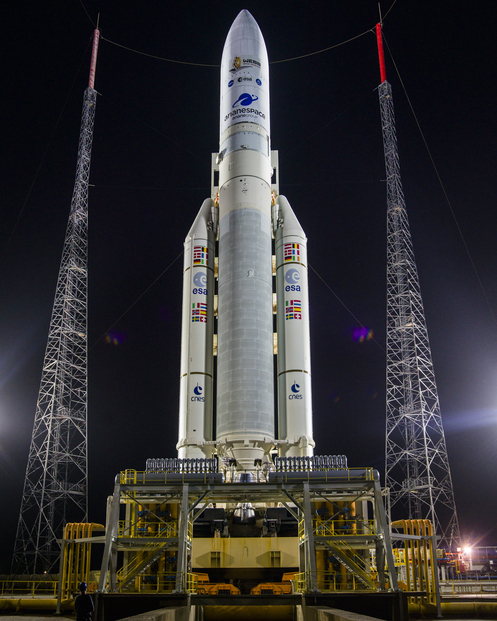
\includegraphics[width=0.8\textwidth]{img/disasters/Ariane_5.jpg}};
            \only<2->{\node [fill=white,rotate=40]  at (0, 0) {\alert{Self-destructed}};}
        \end{tikzpicture}
        \end{center}
        \visible<2->{
        \begin{itemize}
            \item June 1996
            \item Ariane 5 test
            \item 500 million dollar
            \visible<3->{
                \item \alert{floating point conversion error}
            }
        \end{itemize}
        }
    \end{block}
    \end{column}

    \begin{column}{0.3\textwidth}
    \begin{block}{Build an oil rig}
        \begin{center}
            \begin{tikzpicture}
                \node at (0, 0) {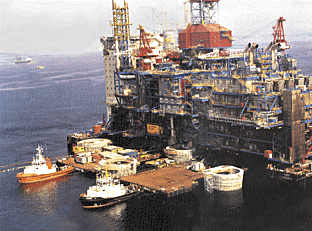
\includegraphics[width=\textwidth]{img/disasters/sleipner.png}};
                \only<2->{\node [fill=white,rotate=40]  at (0, 0) {\alert{Broken and sunken}};}
        \end{tikzpicture}
        \end{center}
        \visible<2->{
        \begin{itemize}
            \item August 1991
            \item Sleipner A offshore platform
            \item 1 billion dollar
            \visible<3->{
            \item \alert{Too crude discretisation}
            }
        \end{itemize}
        }
    \vspace{0.7em}
    \end{block}
    \end{column}

    \begin{column}{0.3\textwidth}
    \begin{block}{Intercept a missile}
        \begin{tikzpicture}
            \node at (0, 0) {
                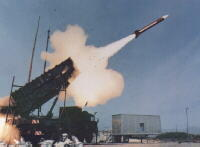
\includegraphics[width=\textwidth]{img/disasters/patriot.jpg}
            };
            \only<2->{\node [fill=white,rotate=40]  at (0, 0) {\alert{Missed Iranian missile}};}
        \end{tikzpicture}
        \visible<2->{
            \vspace{-1.0em}
        \begin{itemize}
            \item February 1991
            \item Patriot missile failure
            \item 28 soldiers killed, 100 injured
            \visible<3->{
            \item \alert{floating point conversion error}
            }
        \end{itemize}
        }
    \end{block}
    \end{column}
    \end{columns}

    \visible<3>{
    \vspace{1.0em}
    \begin{itemize}
            \smaller[2]
        \item See website of Douglas N. Arnold for more details:
            \url{https://www-users.cse.umn.edu/~arnold/disasters/disasters.html}
    \end{itemize}
    }
\end{frame}

\begin{frame}{Ok, so these are the extreme cases, right?}
    \begin{center}
        \larger
        \alert{Brainstorming:} Sources of error in scientific simulations
    \end{center}
    \vspace{3.0em}
    \visible<2>{
    \begin{itemize}
        \item Model
        \item Numerics \textcolor{grey5}{\smaller (discretisation / basis set, algorithm, arithmetic)}
        \item Implementation
        \item Hardware \textcolor{grey5}{\smaller (CPUs have bugs!)}
    \end{itemize}
    }
\end{frame}

\begin{frame}{Motivation in the \matmat group}
    \begin{itemize}
        \item \alert{21st century challenges}:
            \begin{itemize}
                \vspace{-0.3em}
                \item Renewable energy, green chemistry, health care \ldots
            \end{itemize}
        \vspace{0.2em}
        \item Current solutions limited by properties of available materials
            \begin{itemize}
                \vspace{-0.3em}
                \item[$\Rightarrow$] Innovation driven by \alert{discovering new materials}
            \end{itemize}
        \vspace{0.2em}
        \item Crucial tool: \alert{Computational materials discovery}
            \begin{itemize}
                \vspace{-0.3em}
                \item Systematic simulations on \alert{$\simeq 10^4 - 10^6$ compounds}
                \vspace{-0.3em}
                \item Complemented by data-driven approaches
                \vspace{-0.3em}
                \item \alert{Noteworthy share} of world's supercomputing resources
            \end{itemize}
    \end{itemize}
    \vspace{0.2em}
    \definecolor{pgray}{rgb}{0.169,0.169,0.251}
    \begin{center}
        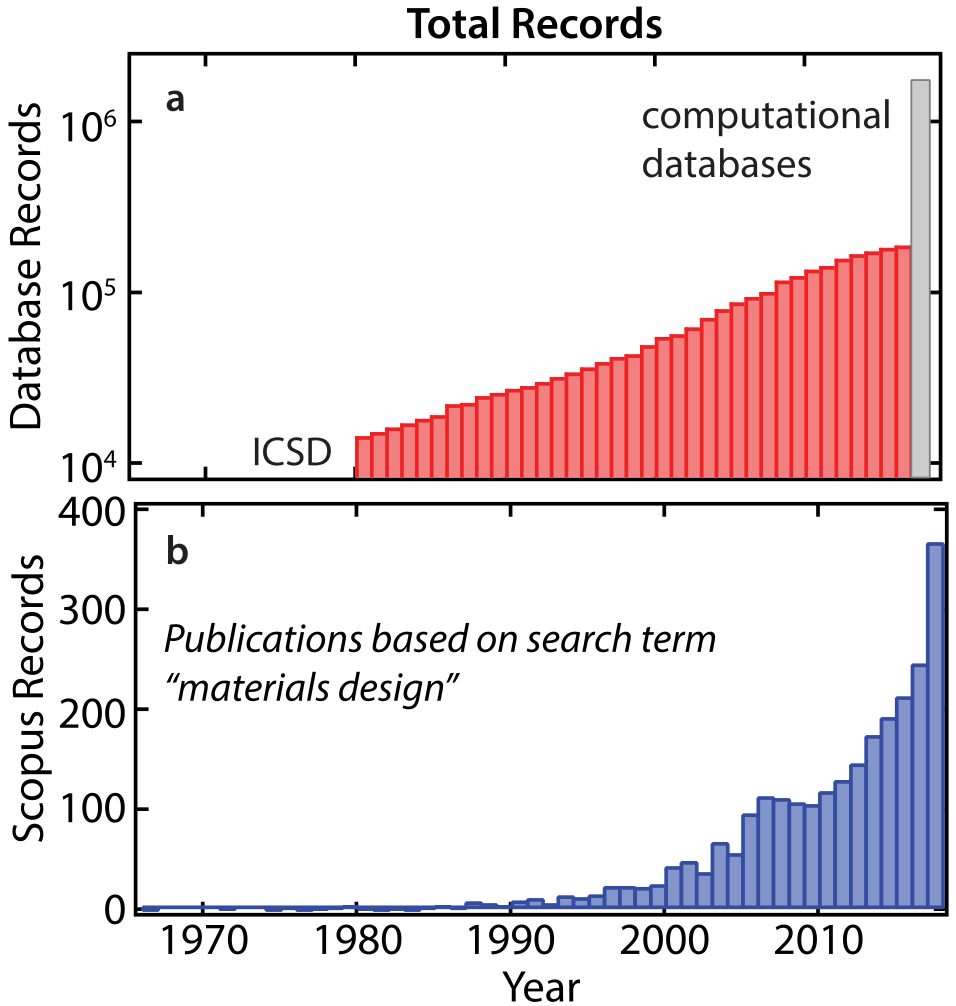
\includegraphics[height=3.3cm]{img/intro/roadmap-growth.png}
        \hspace{1.5em}
        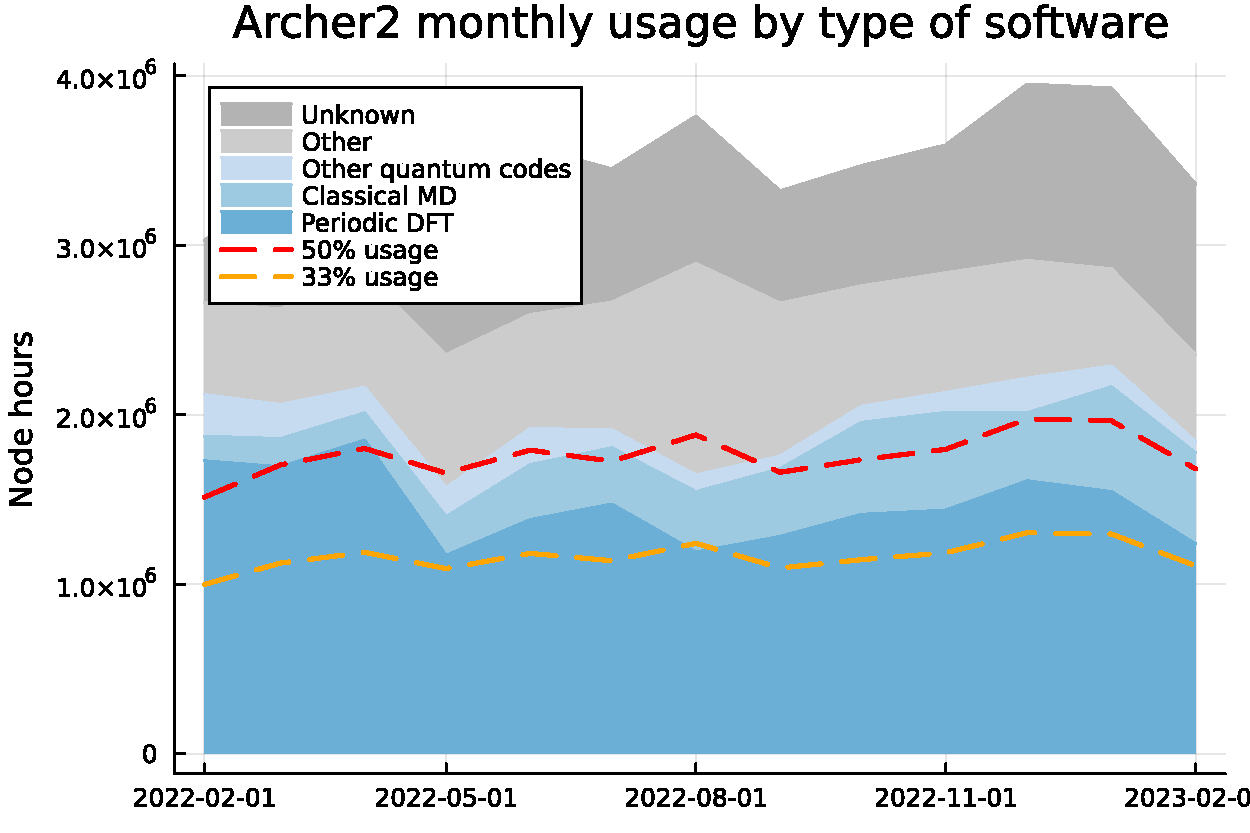
\includegraphics[height=3.3cm]{img/intro/archer_usage.pdf}
    \end{center}
   \vspace{-1.3em}
   \rule{4.5cm}{0.5pt}\\[-0.5em]
   {\tiny \href{http://dx.doi.org/10.1088/1361-6463/aad926}{%
       K. Alberi \textit{et. al.} J. Phys. D, \textbf{52}, 013001 (2019).}}
\end{frame}

\begin{frame}{Sketch of high-throughput workflows}
    \widenframe[4em]{
        \vspace{-0.2em}
        \begin{columns}
        \begin{column}{0.45\textwidth}
        \begin{lpic}[r(2.5cm)]{./img/intro/funnel.png(.125)}
        \lbl[l]{232,153;$\Big\}$\smaller[2.5] DFT PBE stability}
        \lbl[l]{203, 95;\smaller[2.5]DFT PBE band gap}
        \lbl[l]{187, 60;\smaller[2.5]Hybrid-DFT band gap}
        \lbl[l]{175, 25;\smaller[2.5]Beyond DFT}
        \end{lpic}\\[-0.7em]
        {\smaller[2.5] Design funnel for photovoltaic materials}
        \end{column}
        \begin{column}{0.55\textwidth}
        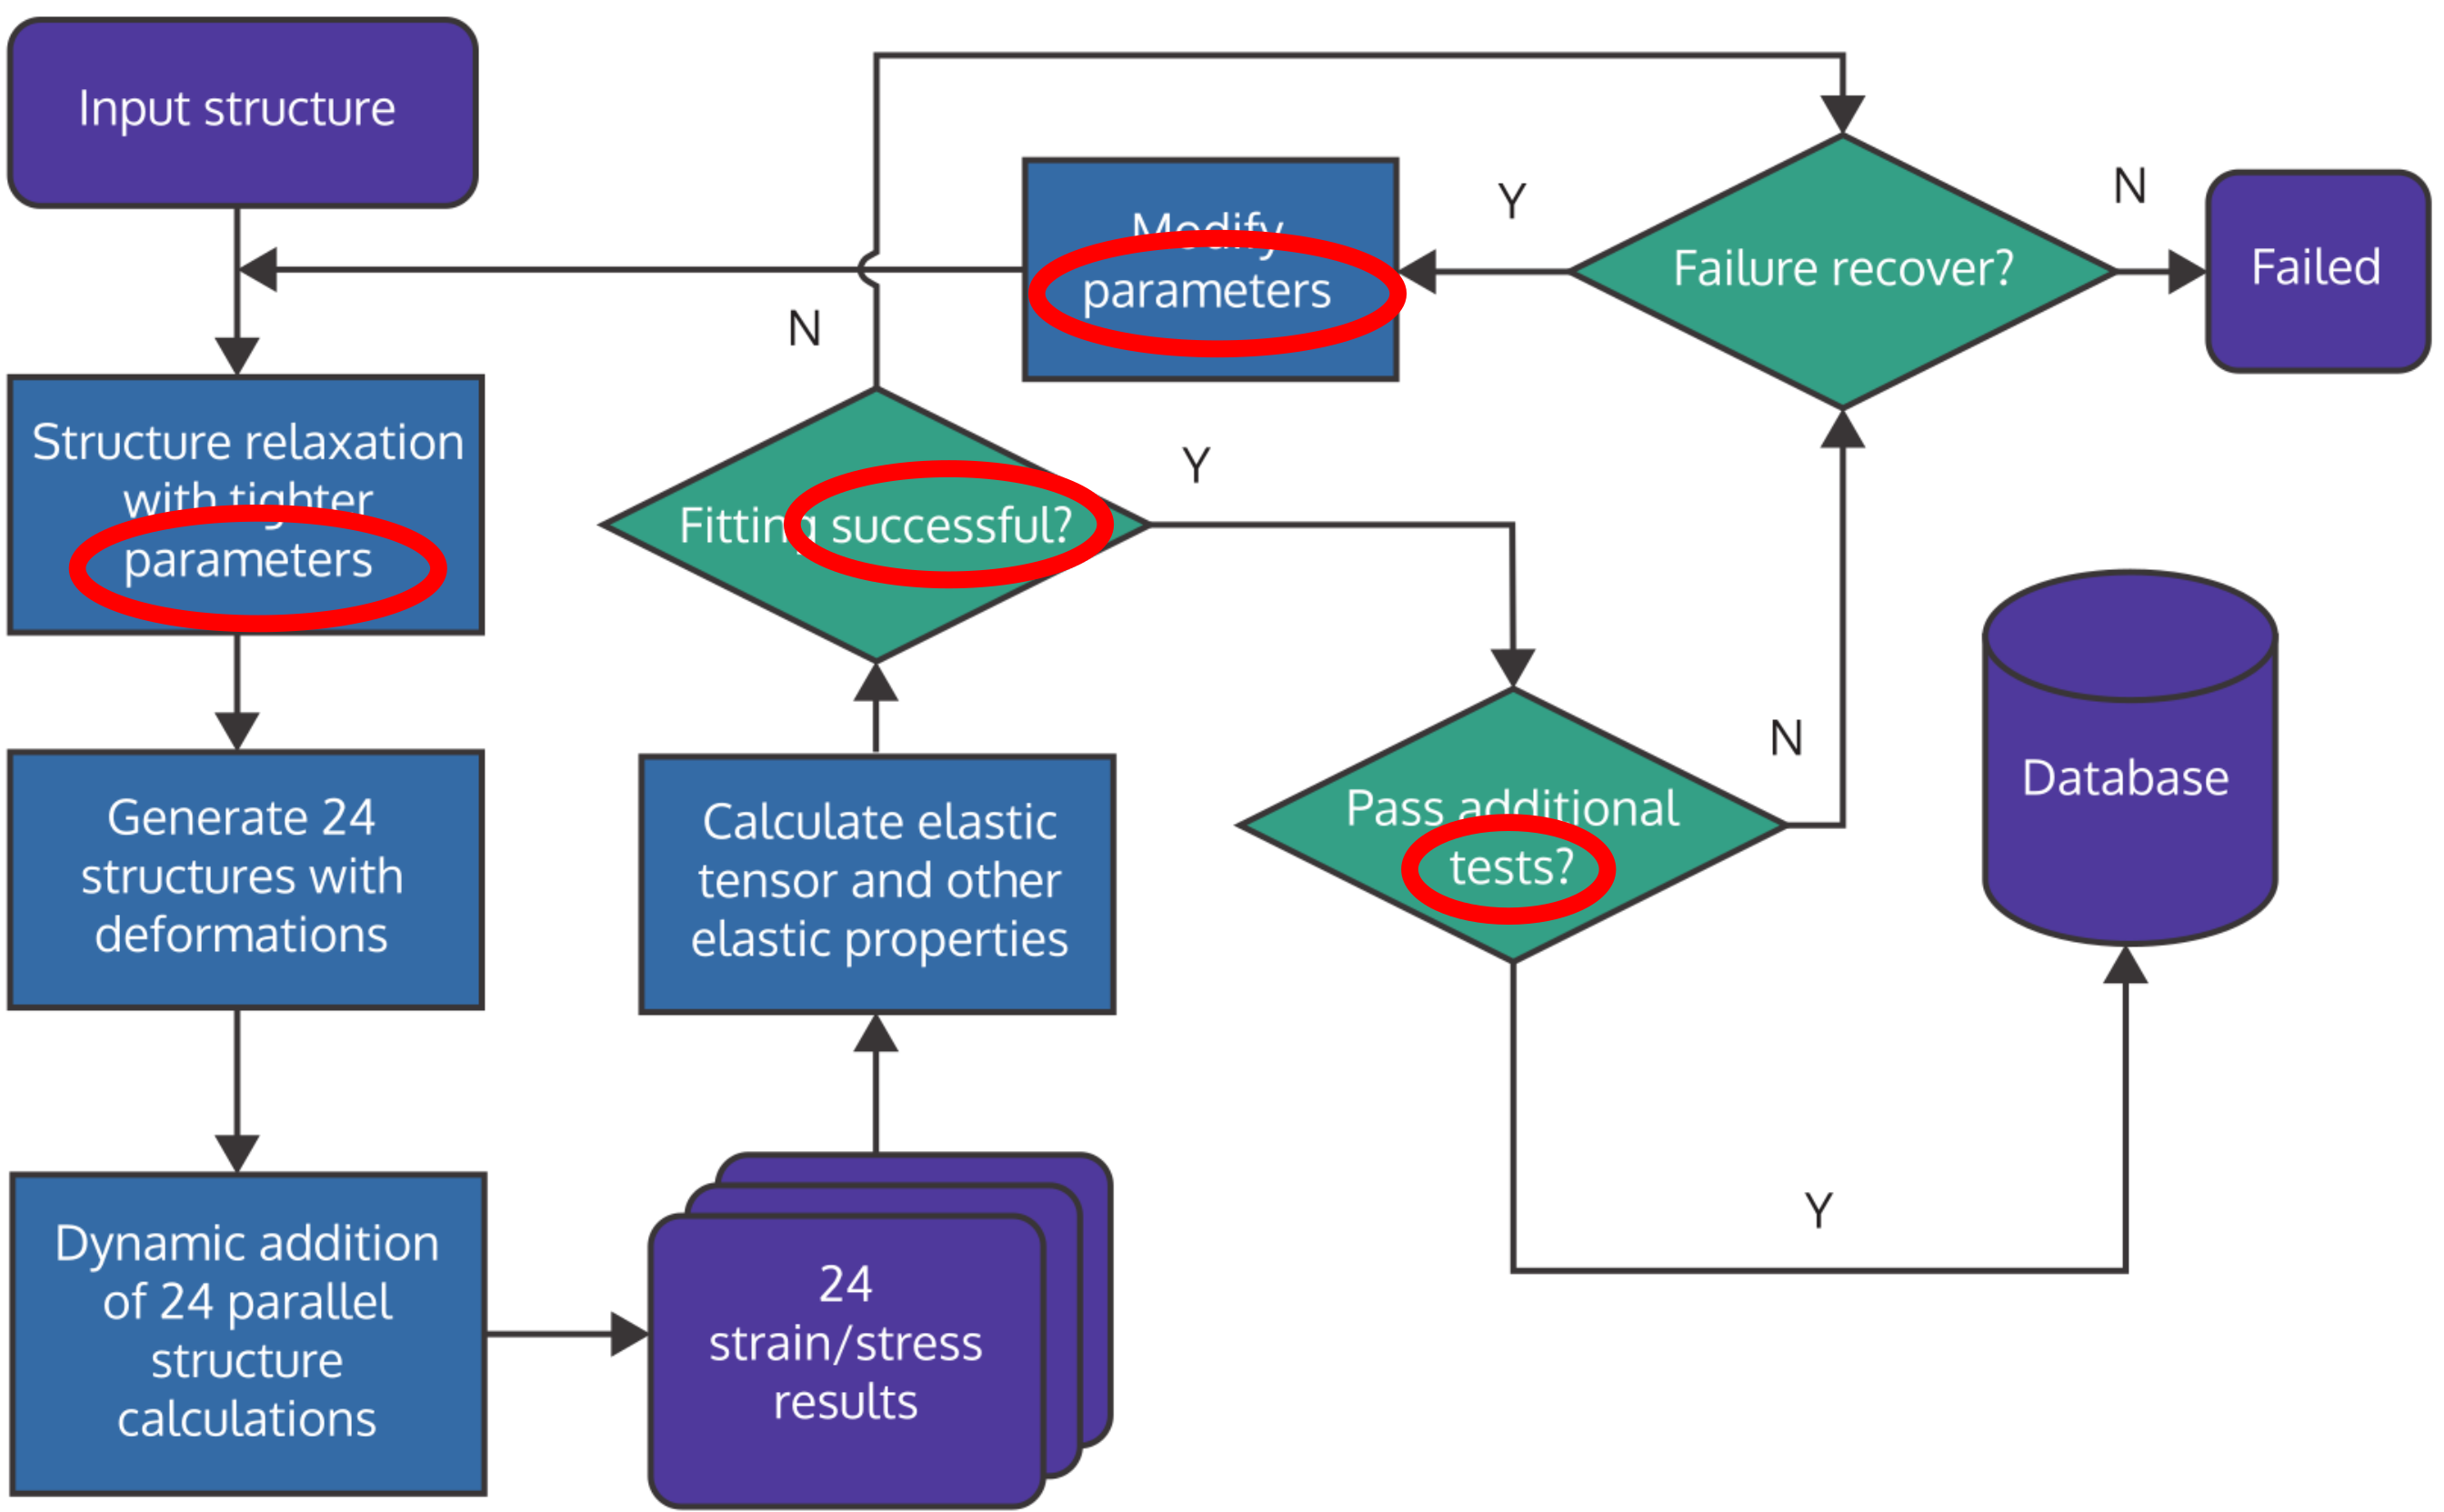
\includegraphics[width=5.0cm]{./img/intro/workflow_edit_parameters.png}%
        \\[-0.5em]
        {\smaller[2.5] Workflow for computing elasticity tensors}
        \end{column}
        \end{columns}
    }
    \vspace{-0.1em}
    \begin{itemize}
        \item Many parameters to choose \textcolor{grey5}{(algorithms, tolerances, models)}
            \begin{itemize}
                \vspace{-0.4em}
                \item Elaborate heuristics: \alert{Failure rate $\simeq 1\%$}
                \vspace{-0.4em}
                \item Still: \alert{Thousands} of failed calculations
                \vspace{-0.4em}
                \item[$\Rightarrow$] \alert{Wasted resources} \& increased human attention
                    \textcolor{grey5}{\smaller (limits througput)}
            \end{itemize}
        % \vspace{0.1em}
        % \item Carbon footprint? More complex design spaces?
        \vspace{0.2em}
        \item \textbf{Goal} in \matmat group: \alert{Self-adapting black-box algorithms}
            \begin{itemize}
                \vspace{-0.4em}
                \item Transform \alert{empirical wisdom} to built-in \alert{convergence guarantees}
                \vspace{-0.4em}
                \item Requires: Uncertainty quantification \& error estimation
                \vspace{-0.4em}
                \item[$\Rightarrow$] Understand \alert{where and how} to spend efforts best
            \end{itemize}
   \end{itemize}
   \vspace{-0.8em}
   \rule{4.5cm}{0.5pt}\\[-0.5em]
   {\tiny G.~Hautier Comput. Mater. Sci. \textbf{164}, 108 (2019);
       L.~Himanen \textit{et. al.} Adv. Science \textbf{6}, 1900808 (2019).}
\end{frame}

\begin{frame}{Broader vision: Robust \& error-controlled simulations}
\begin{itemize}
    \item Error control $=$ \alert{Track simulation uncertainties}:
        \begin{itemize}
            \vspace{-0.30em}
            \item Self-adapting simulations with mathematical guarantees
            \vspace{-0.30em}
            \item Integrate with error propagation efforts for surrogates%
                \footnote{F.~Musil, A.~Grisafi \emph{et. al.} J. Chem. Theo. Comput. \textbf{15}, 2 (2019).}
            \vspace{-0.30em}
            \item [$\Rightarrow$] Byproducts: Data quality control,
                accelerated design%
                % \footnote{G.~Houchins and V.~Viswanathan MRS Bulletin \textbf{44}, 204 (2019).}
        \end{itemize}

    \vspace{0.3em}
    \item Error control $=$ \alert{Learn missing physics}:
        \begin{itemize}
            \vspace{-0.30em}
            \item Data-enhanced models, active learning
            \vspace{-0.30em}
            \item Integration with experiment {\color{grey5} (autonomous discovery)}
            \vspace{-0.30em}
            \item [$\Rightarrow$] Exploit high-fidelity experimental, beyond-DFT data
        \end{itemize}

    \vspace{0.3em}
    \item Error control $=$ \alert{Leverage inexactness}:
        \begin{itemize}
            \vspace{-0.30em}
            \item Error balancing: Optimal adaptive parameter selection
            \vspace{-0.30em}
            \item Randomised methods, selective precision {\color{grey5} (16-bit, FPGA)}
                % Error control and multi-fidelity approaches pretty much unexplored
                % in practical setting
            \vspace{-0.30em}
            \item Multi-fidelity approaches {\color{grey5} (reduced basis, surrogates)}
        \end{itemize}

    \vspace{0.3em}
    \item[$\Rightarrow$] Understand \alert{where and how} to spend efforts best
    \vspace{-0.3em}
    \item[$\Rightarrow$] Realm of mathematical research
\end{itemize}
\vspace{1em}
\end{frame}


\begin{frame}{Questions ?}
    \begin{center}
        \huge{Questions ?}
    \end{center}
\end{frame}

\begin{frame}{Focus of the course: Eigenvalue problems}
    \begin{itemize}
        \item Eigenvalue problems are ubiquitous, e.g.
        \vspace{2em}
        \item \alert{Vibrations of structures}
            \begin{itemize}
                \item Tacoma narrows bridge collapse 1940
                \item London millennium bridge construction flaw
            \end{itemize}
        \vspace{1em}
        \item \alert{Quantum states} \textcolor{grey5}{\smaller (details follow)}
        \vspace{1em}
        \item Tight relation to \alert{linear problems \& PDEs}
            \begin{itemize}
                \item Convergence analysis (CG, iterative methods)
                \item Quantum mechanics
                \item Close relation to solving PDEs
                    \textcolor{grey5}{\smaller (details follow)}
            \end{itemize}
    \end{itemize}
\end{frame}
